\documentclass{book}
\nonstopmode

\usepackage{topology}
\title{Workbook for MAT331-Topology}
\date{Fall 2016}
\author{This workbook, part of the coursework for MAT331-Topology, is based on \cite{viro}.}


\begin{document}
    %\maketitle
    %\tableofcontents
    %%
    %%
    %%
    %\part{General Topology}


\chapter{Structure and Spaces}
Authors: Reilly Noonan Grant, Willie Kaufman, David Kraemer, and Jimin Tan

\section{Set-Theoretic Digression: Sets}
\subsection{Sets and Elements}%1'1
\subsection{Equality of Sets}%1'2
\subsection{The Empty Set}%1'3
\subsection{Basic Set of Numbers}%1'4

\subsection{Describing a Set By Listing Its Elements}%1'5
				\begin{minorEx}%1.1
					What is $ \{\emptyset\} $? How many elements does it contain?
				\end{minorEx}
				\begin{proof}[Answer]
					This is a set made up of the empty set, it contains one element.
				\end{proof}
				\begin{minorEx}%1.2
                Which of the following formulas are correct:
				\begin{enumerate}
                \item $\emptyset \in \{\emptyset, \{\emptyset\}\}$ is correct
                \item $\{\emptyset\} \in \{\{\emptyset\}\}$ is correct
                \item $\emptyset \in \{\{\emptyset\}\}$ is incorrect
                \end{enumerate}
                Primary author: Willie Kaufman
				\end{minorEx}
				\begin{minorEx}%1.3
					Yes, \{\{$\emptyset$\}\} contains just one element. \newline
                    Primary author: Willie Kaufman
				\end{minorEx}
				\begin{minorEx}%1.4
					How many elements do the following sets contains?
				\end{minorEx}
                \begin{enumerate}
					\item $\{1,2,1 \}$; 2 elements
					\item $\{ 1,2,\{1,2\} \}$; 3 elements
					\item $\{\{ 2 \} \}$; 1 element
					\item $\{ \{1 \}, 1\}$; 2 elements
					\item $\{ 1, \emptyset \}$; 2 elements
					\item $\{ \{ \emptyset \}, \emptyset \}$; 2 elements
					\item $\{ \{ \emptyset\}, \{\null\} \}$; 1 element
					\item $\{x, 3x-1 \} \text{for some } x\in \RR$; 1 element if $x = \frac{1}{2}$, and 2 elements for all for all values of $x$
                \end{enumerate}
                Primary author: Reilly Noonan Grant
                \begin{minorEx}
                (a) : $\{0, 1, 2, 3, 4\}$
                
                (b) : $\emptyset$
                
                (c) : $\{-1, -2, -3, \cdots\}$
                \end{minorEx}

\subsection{Subsets}%1'6
				\begin{majorEx}%1.A
					Let a set $ A $ have $a$ elements, and let a set $B$ have $b$ elements. Prove that if $A \subset B $, then $a\leq b$.
				\end{majorEx}
				\begin{proof}
					Suppose  $ A $ is a set made up of $a$ elements, and $B$ is a set made up of $b$ elements. Suppose $a > b$; then there must be some element $x \in A$ that satisfies $x \notin B$. This implies that $A \not\subset B$, as $x$ is not a member of $B$. By the contrapositive, we obtain the desired result.
				\end{proof}


\subsection{Properties of Inclusion}%1'7
				\begin{majorEx}[Reflexivity of Inclusion]%1.B
                Any set includes itself: $A \subset A$ holds true for any $A$.
				\end{majorEx}
                \begin{proof}
                  We first let $A$ be an arbitrary Set. Suppose that $A$ is the empty set. We would then see that as $A$ doesn't have any elements, that it is vacuously true that every element of $A$ is in $A$, and thus  $A \subset A$. Now suppose that $A$ is non empty. Let $a \in A$ be arbitrary. We see that $a \in A$, and as $a$ was arbitrary, we know that this is true for all elements of $A$, and thus $A \subset A$. As $A$ was arbitrary, and $A \subset A$ for all cases, we see that $A \subset A$ holds true for any $A$.
                \end{proof}
                Primary author: Reilly Noonan Grant
				\begin{majorEx}%1.C
					\textbf{\textit{The Empty Set Is Everywhere.}} The inclusion $\emptyset \subset A$ holds true for any A. In other words, the empty set is present in each set as a subset.
                     \begin{proof}
                    Assume that $\emptyset \subset A$ does not hold, by defintion of inclusion, there exist at least one element $a \in \emptyset$ such that $a \not\in A$. Since $\emptyset$ does not contain any element, we have a contradiction, and the statement above is true.
                    \end{proof}
                    Primary author: Jimin Tan
				\end{majorEx}
				\begin{majorEx}%1.D
					If A , $B$, and $C$ are sets, $A \subset B$, and $B \subset C$, then $A \subset C$. 
				\end{majorEx}
                \begin{proof}
                Let $A$, $B$, and $C$ be arbitrary sets such that $A \subset B$ and $B \subset C$. If $A$ is the empty set, it is true that $A \subset C$. If $A$ is nonempty, choose an arbitrary element $a \in A$. Because $A \subset B$, we know that $a \in B$, and similarly because  $B \subset C$, $a \in C$. Since $a$ was arbitrary, $A \subset C$. \newline
                \end{proof}
      		 Primary author: Willie Kaufman

\subsection{To Prove Equality of Sets, Prove Two Inclusions}%1'8
            	\begin{majorEx} % 1.E
                	[Criterion of Equality for Sets.]
                    $A = B$ if and only if $A \subset B$ and $B \subset A$.
                \end{majorEx}
                \begin{proof}
					Let $A$ and $B$ be arbitrary sets. Let us first suppose that $A = B$. We show that $A \subset B$ and $B \subset A$. Let $x \in A$ be arbitrary. Since $A = B$, they have the same elements; since $x$ is an element of $A$, $x$ is an element of $B$. Hence, $A \subset B$. A similar argument establishes that $B \subset A$.
                    
                    We now establish the converse of the previous claim via contraposition. Suppose that it is not the case that $A \subset B$ and $B \subset A$; without loss of generality, we shall assume that $A \not\subset B$. Then there necessarily exists an element $x \in A$ satisfying $x \notin B$. As such, it is not the case that $A$ and $B$ contain the same elements, since $B$ does not contain $x$. Hence, $A \ne B$. By the contrapositive, this establishes the converse.
				\end{proof}

\subsection{Inclusion Versus Belonging}%1'9
            \begin{majorEx}%1.F
            $x \in A$ if and only if $\{x\} \subset A$.
            \end{majorEx}

\begin{proof} We will first show that if $\{x\} \subset A$, then $x \in A$. We can see that as $\{x\}$ is a set described by listing all of its elements, that $x \in \{x\}$. We also see that
as $\{x\} \subset A$, that all of the elements of $\{x\}$ are also elements of $A$, and thus $x \in A$. We thus know that if $\{x\} \subset A$, then $x \in A$.

We will now show that if $x \in A$, then $\{x\} \subset A$. We can see that as $\{x\}$ is a set described by listing all of its elements, that $x$ is the only element in $\{x\}$.
We also see that as $x \in A$, that all elements of $\{ x\}$ belong to $A$, and thus $\{x\} \subset A$. We now can see that $x \in A$ if and only if $\{x\} \subset A$.
\end{proof}
Primary author: Reilly Noonan Grant			
            \begin{majorEx}%1.G
            \textbf{\textit{Non-Reflexivity of Belonging.}} Construct a set $A$ such that $A \not\in A$.
            The example, $\{1\} \not\in \{1\}$ shows the statement above. The set that contains $\{1\}$ is $\{\{1\}\}$.
                    Primary author: Jimin Tan            
                    \end{majorEx}
            
\begin{majorEx}%1.H
            \textbf{\textit{Non-Transitivity of Belonging.}} Construct three sets A, B, and C such that $A \in B$ and $B \in C$, but $A \not \in C$.
            \newline $A = \{1\}$
            \newline $B = \{\{1\}, 2\}$
            \newline $C = \{\{\{1\}, 2\}, 3\}$
            \newline
            \end{majorEx}
            
Primary author: Willie Kaufman

\subsection{Defining a Set by a Condition (Set-Builder Notation)}%1'10

\subsection{Intersection and Union}%1'11

\begin{majorEx} % 1.I
    [Commutativity of $\cap$ and $\cup$]
    For any two sets $A$ and $B$, we have
    \[
        A \cap B = B \cap A \quad \text{and} \quad A \cup B = B \cup A.
    \]
\end{majorEx}

\begin{proof}
    For our proof we rely on the commutativity of logical operators, which can
    be verified via truth tables. Namely, we have
    \[
        \alpha \text{ and } \beta = \beta \text{ and } \alpha \quad \text{and}
        \quad \alpha \text{ or } \beta = \beta \text{ or } \alpha, 
    \]
    where $\alpha$ and $\beta$ are arbitrary statements. We will show that the
    statements about intersections and unions reduce to statements with ``and''
    and ``or'' operators, respectively.

    Let $A$ and $B$ be arbitrary sets. Then $x \in A \cap B$ if and only if $x
    \in A$ and $x \in B$, which holds if and only if $x \in B$ and $x \in A$,
    which holds if and only if $x \in B \cap A$. This establishes via
    double-containment that $A \cap B = B \cap A$.

    Similarly, $x \in A \cup B$ if and only if $x \in A$ or $x \in B$, which
    holds if and only if $x \in B$ or $x \in A$, which holds if and only if $x
    \in B \cup x \in A$. This establishes via double-containment that $A \cup B
    = B \cup A$.
\end{proof}

Primary author: David Kraemer.

\begin{minorEx}%1.6
    Prove that for any set $A$ we have $ A \cap A = A$, $A \cup A = A$, $A \cup
    \emptyset = A$, and $A \cap \emptyset = \emptyset$.
\end{minorEx}

\begin{proof}
    Let $A$ be an arbitrary set. If $A$ is the empty set, each of these is
    true. So we consider when A is not the emptyset. Choose an arbitrary
    element $a \in A$. This element is in $A \cap A$ by the definition of
    intersection, as it belongs to both $A$ and $A$. This element is also in
    $A \cup A$ by the definition of union, as it belongs to at least one of
    $A$ and $A$. This element is in $A \cup \emptyset$, as it belongs to at
    least one of $A$ and $\emptyset$. This element is not in $A \cap
    \emptyset$, as it does not belong to both $A$ and $\emptyset$. Since $a$
    was arbitrary, each element of $A$ will be in $A \cup A$, $A \cap A$,
    and $A \cup \emptyset$, and no elements of $A$ will be in $A \cap
    \emptyset$. No elements that do not belong to $A$ could be in any of
    these sets, so combining these two facts requires that $A \cup A$, $A
    \cap A$, and $A \cup \emptyset$ each equal $A$ and $A \cup \emptyset =
    \emptyset$.
\end{proof}
Primary author: Willie Kaufman

\begin{minorEx}%1.7
    Prove that for any sets $A$ and $B$ we have 
    $$
    A \subset B, \hspace{15pt} \text{\normalfont iff } \hspace{15pt} A \cap B =
    A, \hspace{15pt} \text{\normalfont iff } \hspace{15pt} A \cup B = B
    $$
\end{minorEx}

\begin{proof}
            We will break this chain if and only if statement into two parts and then prove them separately.
            
            To begin with, we want to show that $A \subset B, $  if and only if $A \cap B = A$.
            For if and only if statement, we need to prove it in both directions. For the forward direction, assume that $A \subset B$ and let $x \in A$, since $A \subset B$, we know that $x \in B$ by definition of inclusion. We have $x \in A$ and $x \in B$, so $x \in A \cap B$. Since $A \cap B \subset A$ by definition of intersection, we have $$A \cap B = A$$
            Then, we consider the backward direction, assume that $A = A \cap B$ and let $x \in A$, since $A \subset A \cap B$, we have $x \in A$ and $x \in B$. Hence, we have $$A \subset B$$
            
            Now we want to prove the second if and only if statement which is $A \cap B = A \hspace{5pt} \text{\normalfont iff } \hspace{5pt} A \cup B = B.$ 
            
            We start with the forward. Assume that $A \cap B = A$ and let $x \in A \cup B$, by definition, we know $x \in A$ or $x \in B$. If $x \in A$, since $A \subset A \cap B$, $x \in B$. Since $B \subset A \cup B$, we have: $$A \cup B = B$$
            
            Backward direction:
            Let $x \in A$, since $A \cup B \subset B$, $x \in B$. We have whenever $x \in A$, $x \in B$, so $x \in A \cap B$ and $A \subset A \cap B$. Since $A \cap B \subset A$, we have $$A \cap B = A$$
            \end{proof} 
                    Primary author: Jimin Tan

  \begin{majorEx}%1.J
            Associativity of $\cap$ and $\cup$. For any sets $A$, $B$,
            and $C$, we have $$(A \cap B) \cap C = A \cap (B \cap C)$$
            and $$(A \cup B) \cup C = A \cup (B \cup C)$$
          \end{majorEx}
            \begin{proof}
            Let $A$, $B$, and $C$ be arbitrary sets. First, consider the associativity of $\cap$. In the case of intersection, if any of $A$, $B$, or $C$ are $\emptyset$, the top claim is true, as both evaluate to the emptyset. So consider the case where none of $A$, $B$, or $C$ are the emptyset. Choose an arbitrary element $a \in A \cup B \cup C$. Only elements in $A \cup B \cup C$ will be in the intersection of these sets, so we can ignore other elements; if the two sets we are considering contain exactly the same elements from these sets, they will be the same. $a \in (A \cap B) \cap C$ iff $a \in A \cap B$ and $a \in C$ by the definition of intersection. $a\in A \cap B$ iff $a \in A$ and $a \in B$ by the definition of intersection. Combining these logically, $a \in (A \cap B) \cap C$ iff it is an element of $A$, $B$, and $C$. Now considering the right side of the equation, $a \in A \cap (B \cap C)$ iff it is in both $A$ and $B \cap C$ by the definition of intersection. $a$ is in $B \cap C$ iff it is in $B$ and $C$ by the definition of intersection. Combining these logically, we have that $a \in A \cap (B \cap C)$ iff $a \in A$, $a \in B$ and $a \in C$. We know that $a \in (A \cap B) \cap C$ iff $a \in A$ and $a \in B$ and $a \in C$ iff $a \in A \cap (B \cap C)$, or $a \in (A \cap B) \cap C$ iff $a \in A \cap (B \cap C)$. Since $a$ was arbitrary, these sets must be the same. \newline
            Second, consider the associativity of $\cup$. If all of $A$, $B$, and $C$ are $\emptyset$, both the left and right hand sides of the equation evaluate to $\emptyset$, and so the bottom claim is true. So consider the case where $A \cup B \cup C$ is nonempty. Choose an arbitrary element $a \in A \cup B \cup C$. Only elements in $A \cup B \cup C$ will be in the union of these sets, so we can ignore other elements; if the two sets we are considering contain exactly the same elements from these sets, they will be the same. $a \in (A \cup B) \cup C$ iff $a \in (A \cup B)$ or $a \in C$ by the definition of union. $a \in (A \cup B)$ iff $a \in A$ or $a \in B$ by the definition of union. Combining these logically, $a \in (A \cup B) \cup C$ iff $a \in A$, $a \in B$ or $a \in C$. Now consider the right hand side of the equation. $a \in A \cup (B \cup C)$ iff $a \in A$ or $a \in B \cup C$ by the definition of union.  $a \in B \cup C$ iff $a \in B$ or $a \in C$ by the definition of union. Combining these logically, $a \in A \cup (B \cup C)$ iff $a \in A$, $a \in B$, or $a \in C$. We know that $a \in (A \cup B) \cup C$ iff $a \in A$, $a \in B$, or $a \in C$ iff $a \in (A \cup B) \cup C$. Since $a$ was arbitrary, these sets must be the same.
            \end{proof}

            Primary author: Willie Kaufman

\begin{majorEx}%1.K
    The notions of intersection and union of an arbitrary collection of sets
    generalize the notions of intersection and union of two sets: for $\Gamma =
    \{A, B\}$, we have 
    $$
    \bigcap_{C \in \Gamma} C = A \cap B \hspace{5pt} \text{\normalfont and}
    \hspace{5pt} \bigcup_{C \in \Gamma} C = A \cup B
    $$
\end{majorEx}

\begin{proof}
            
            We will discuss the intersection of multiple sets first.
            
            Let $x \in \bigcap_{C \in \Gamma}$ and assume we can list all element like $C_0, C_1 \cdots, C_n \cdots$, we have $x \in C_0 \cap C_1 \cdots \cap C_n$ by definition. Since there are only two sets in $\Gamma$, which are $A, B$, $x \in A \cap B$. We have $\bigcap_{C \in \Gamma} \subset A \cap B$. Let $y \in A \cap B$. Since $A$ and $B$ are the only two elements in $\Gamma$, we have $y \in \bigcap_{C \in \Gamma}$, and $A \cap B \subset \bigcap_{C \in \Gamma}$. Then we have $$A \cap B = \bigcap_{C \in \Gamma}$$
            
            Union:
            
            Let $x \in \bigcup_{C \in \Gamma}$ and assume we can list all element like $C_0, C_1 \cdots, C_n \cdots$, we have $x \in C_0 \cup C_1 \cdots \cup C_n$. Since $A$ and $B$ are the only two sets in $\Gamma$, we have $x \in A \cup B$ and $\bigcup_{C \in \Gamma} \subset A \cup B$. Let $y \in A \cup B$, since $A$ and $B$ are the only two sets in $\Gamma$, we have $y \in \bigcup_{C \in \Gamma}$, and $A \cup B \subset \bigcup_{C \in \Gamma}$. Then we have $$A \cup B = \bigcup_{C \in \Gamma}$$
            \end{proof}
                    Primary author: Jimin Tan


\begin{minorEx}%1.8
    [Riddle]
    How are the notions of system of equations and intersection of sets related
    to each other?
\end{minorEx}

\begin{proof}
    [Answer]
    If $E_1, E_2, \ldots, E_n$ are a system of equations and $S_1, S_2, \ldots,
    S_n$ are the solution sets corresponding to each equation, then the set
    \[
        S = \bigcap_{i=1}^{n} S_i
    \]
    is the solution to the system of equations, as any solution $s \in S$ solves
    each equation $E_i$ simultaneously.
\end{proof}

Primary author: David Kraemer

\begin{majorEx}[Two Distributitivites]%1.L
    For any sets $A$, $B$, and $C$, we have
    \begin{align*}
        (A \cap B) \cup C &= (A \cup C) \cap (B \cup C) \\
        (A \cup B) \cap C &= (A \cap C) \cup (B \cap C)
    \end{align*}
\end{majorEx}
\begin{proof}
    These properties follow from unpacking the definitions of set union and
    intersection, as well as from recalling the distributive properties of
    logical operators:
    \begin{align*}
        (\alpha \text{ and } \beta) \text{ or } \gamma &\iff (\alpha \text{ or }
        \gamma) \text{ and } (\beta \text{ or } \gamma) \\
        (\alpha \text{ or } \beta) \text{ and } \gamma &\iff (\alpha \text{ and
        } \gamma) \text{ or } (\beta \text{ and } \gamma).
    \end{align*}
    We first show  $(A \cap B) \cup C = (A \cup C) \cap (B \cup C)$. We have
    that
    \[
        x \in (A \cap B) \cup C
    \]
    if and only if either 
    \[
        x \in A \cap B \text{ or } x \in C,
    \] 
    which holds if and only if
    \[
        (x \in A \text{ and } x \in B) \text{ or } x \in C,
    \]
    which holds if and only if 
    \[
        (x \in A \text{ and } x \in C) \text{ or } (x \in B \text{ and } x \in C), 
    \]
    which holds if and only if
    \[
        (x \in A \cap C) \text{ or } (x \in B \cap C),
    \]
    which holds if and only if
    \[
        x \in (A \cap C) \cup (B \cap C).
    \]

    We now show  $(A \cup B) \cap C = (A \cap C) \cup (B \cap C)$. We have that
    \[
        x \in (A \cup B) \cap C
    \]
    if and only if either 
    \[
        x \in A \cup B \text{ and } x \in C,
    \] 
    which holds if and only if
    \[
        (x \in A \text{ or } x \in B) \text{ and } x \in C,
    \]
    which holds if and only if 
    \[
        (x \in A \text{ or } x \in C) \text{ and } (x \in B \text{ or } x \in C), 
    \]
    which holds if and only if
    \[
        (x \in A \cup C) \text{ and } (x \in B \cup C),
    \]
    which holds if and only if
    \[
        x \in (A \cup C) \cap (B \cup C).
    \]
    These equivalencies establish the claim.
\end{proof}

Primary author: David Kraemer

\begin{majorEx}
    Draw a Venn diagram illustrating (2). Prove (1) and (2) by tracing all
    details of the proofs in the Venn diagrams. Draw Venn diagrams illustrating
    all formulas below in this section.
\end{majorEx}

\begin{proof}[Answer]
    Demonstration of  $(A \cup B) \cap C = (A \cap C) \cup (B \cap C)$:
    \[
        \centerimage{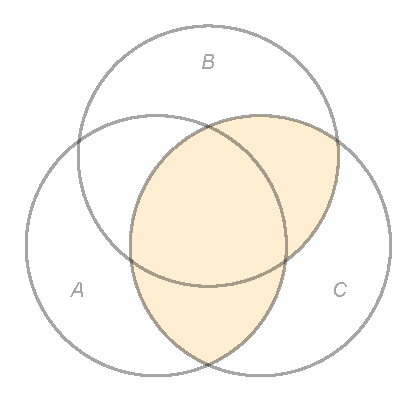
\includegraphics[width=0.2\textwidth]{images/venn1.pdf}}
        =
        \centerimage{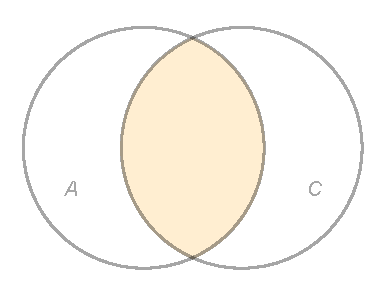
\includegraphics[width=0.2\textwidth]{images/venn2.pdf}}
        \cup
        \centerimage{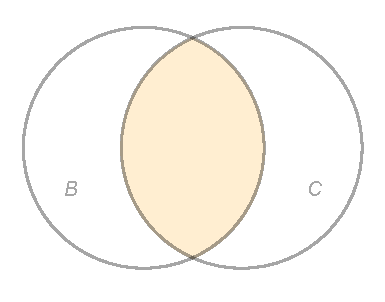
\includegraphics[width=0.2\textwidth]{images/venn3.pdf}}
    \]
    Demonstration of $A \cap \bigcup_{B \in \Gamma} B = \bigcup_{B \in \Gamma}
    (A \cap B)$, with $|\Gamma| = 3$.
    \[
        \centerimage{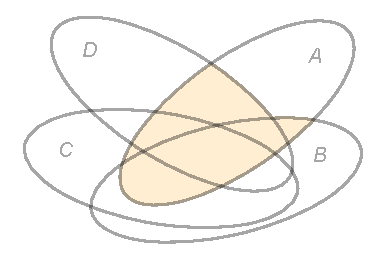
\includegraphics[width=0.2\textwidth]{images/venn4.pdf}} 
        =
        \centerimage{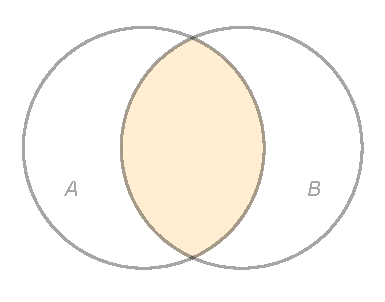
\includegraphics[width=0.2\textwidth]{images/venn5.pdf}} 
        \cup
        \centerimage{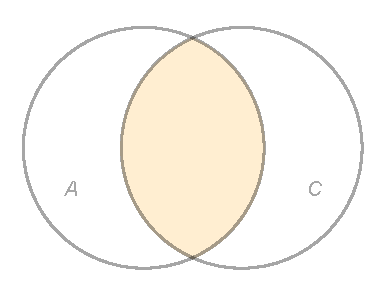
\includegraphics[width=0.2\textwidth]{images/venn6.pdf}} 
        \cup
        \centerimage{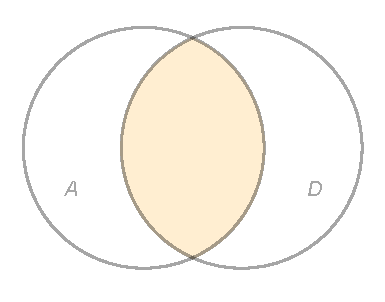
\includegraphics[width=0.2\textwidth]{images/venn7.pdf}} 
    \]
    Demonstration of $A \cup \bigcap_{B \in \Gamma} B = \bigcap_{B \in \Gamma}
    (A \cup B)$, with $|\Gamma| = 3$.
    \[
        \centerimage{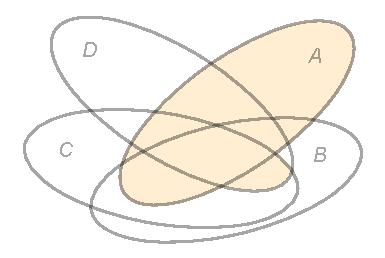
\includegraphics[width=0.2\textwidth]{images/venn11.pdf}} 
        =
        \centerimage{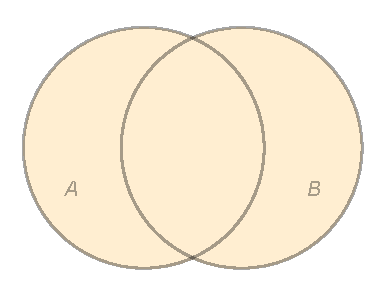
\includegraphics[width=0.2\textwidth]{images/venn8.pdf}} 
        \cap
        \centerimage{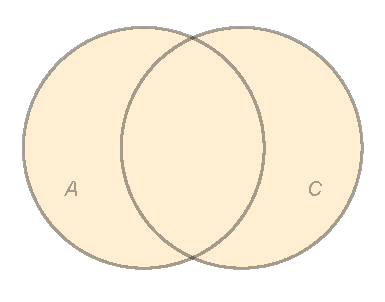
\includegraphics[width=0.2\textwidth]{images/venn9.pdf}} 
        \cap
        \centerimage{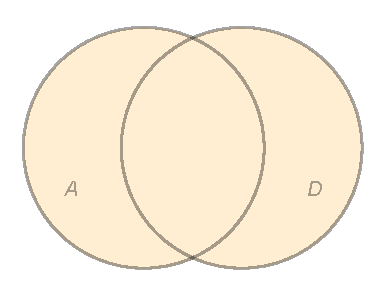
\includegraphics[width=0.2\textwidth]{images/venn10.pdf}} 
    \]
\end{proof}

Primary author: David Kraemer.

\begin{minorEx}[Riddle]%1.9
    Generalize Theorem 1.L to the case of arbitrary collections of sets.
\end{minorEx}

\begin{proof}
    (See 1.N) Let $A$ be a set and let $\Gamma$ be a set consisting of sets,
    then we have 
    $$
    A \cap  \bigcup_{B\in \Gamma} B = \bigcup_{B\in \Gamma} (A \cap B)\text{
    and  } A \cup \bigcap_{B\in \Gamma} B = \bigcap_{B\in \Gamma} (A \cup B)
    $$
\end{proof}
Primary author: Reilly Noonan Grant

\begin{majorEx}[Yet Another Pair of Distributivities]%1.N 
    Let $A$ be a set and let $\Gamma$ be a set consisting of sets, then we have

    $$
    A \cap  \bigcup_{B\in \Gamma} B = \bigcup_{B\in \Gamma} (A \cap B)\text{
    and  } A \cup \bigcap_{B\in \Gamma} B = \bigcap_{B\in \Gamma} (A \cup B)
    $$
\end{majorEx}
\begin{proof}
    We will first show that $A \cap \bigcup_{B\in \Gamma} B = \bigcup_{B\in
    \Gamma} (A \cap B)$ using double containment. 

    First let $x \in A \cap \bigcup_{B\in \Gamma} B$ be arbitrary. We see that
    $$
        x \in A \text{ and } x\in B
    $$ 
    for some $B \in \Gamma$.  We thus know that for some $B$, 
    $$
        x\in (A \cap B)
    $$ 
    We now can see that as 
    $$
        \bigcup_{B\in \Gamma} (A \cap B)
    $$ 
    contains every $(A \cap B)$, we know that 
    $$
        x \in \bigcup_{B\in \Gamma} (A \cap B)
    $$ 
    As $x$ was arbitrary, we know that 
    $$
        A \cap \bigcup_{B\in \Gamma} B \subseteq 
        \bigcup_{B\in \Gamma} (A \cap B).
    $$ 

    We now let $x \in \bigcup (A \cap B)$ be arbitrary.  We see that 
    $$
        x \in A \text{ and } x \in B
    $$ 
    for some $B\in \Gamma$. 
    We also see that as $B\in \Gamma$, that 
    $$
        B \subset \bigcup_{B\in \Gamma} B
    $$ 
    and thus $x \in A \text{ and } x \in \bigcup_{B\in \Gamma}$.  We now can see
    that this only holds if 
    $$
        x \in A \cap \bigcup_{B\in \Gamma}
    $$ 
    and thus as $x$ was arbitrary 
    $$
        A \cap \bigcup_{B\in \Gamma} B \supseteq \bigcup_{B\in \Gamma} (A \cap
        B).
    $$ 
    We now can see by double containment, that $A \cap \bigcup_{B\in \Gamma} B =
    \bigcup_{B\in \Gamma} (A \cap B)$.

    We will now show that 
    $$
        A \cup \bigcap_{B\in \Gamma} B = \bigcap_{B\in \Gamma} (A \cup B)
    $$ 
    by double containment.

    We first let $x \in A \cup \bigcap_{B\in \Gamma} B$ be arbitrary.  We see that 
    $$
        x \in A \text{ or } x \in \bigcap_{B\in \Gamma} B
    $$ 
    We now suppose that $x \in A$. We would then see that $x \in A \cup B$ for
    any $B$, and thus 
    $$
        x \in \bigcap_{B\in \Gamma} (A \cap B)
    $$

    Now suppose that $x \notin A$. We would then see that 
    $$
        x \in \bigcap_{B\in \Gamma} B
    $$ 
    and if $x$ is in some $B$, we know that it would also be in $A
    \cup B$, so thus, we would know that 
    $$
        x \in \bigcap_{B\in \Gamma} (A \cup B)
    $$

    As $x$ was arbitrary, we know that 
    $$
        A \cup \bigcap_{B\in \Gamma} B \subseteq \bigcap_{B\in \Gamma} (A \cup B)
    $$

    We now let $x \in \bigcap_{B\in \Gamma} (A \cup B)$ be arbitrary.
    We can see
    that $x \in A$ or $x \in B$ for every $B \in \Gamma$.  Suppose $x
    \in A$. It would then be the case that $x \in A \cup
    \bigcap_{B\in\Gamma} B$ as $x \in A$.
    Now, suppose that $x \notin A$ we would then have that $x \in
    \bigcap_{B\in\Gamma} B$ as $x \in \bigcap_{B\in\Gamma} (A \cap B)$, and $x
    \notin A$. We thus see that as $x$ was arbitrary, that 
    $$
        A \cup \bigcap_{B\in \Gamma} B \supseteq \bigcap_{B\in \Gamma} (A \cup
        B).
    $$
    and thus 
    $$
        A \cup \bigcap_{B\in \Gamma} B = \bigcap_{B\in \Gamma} (A \cup B)
    $$
    We can now see that
    $$
        A \cap  \bigcup_{B\in \Gamma} B = \bigcup_{B\in \Gamma} (A \cap B)\text{
        and  } A \cup \bigcap_{B\in \Gamma} B = \bigcap_{B\in \Gamma} (A \cup B)
    $$

\end{proof}
Primary author: Reilly Noonan Grant
\subsection{Different Differences}%1'12
			\begin{minorEx}%1.10
            Prove that for any two sets $A$ and $B$ their union $A \cup B$ is the union of the following three sets: $A \setminus B$, $B \setminus A$, and $A \cap B$, which are pairwise disjoint.
            \begin{proof}Let $A$, $B$ and $C$ be arbitrary sets. For an arbitrary value $a$, $a \in A \cup B$ iff $a \in A$ or $a \in B$. This is equivalent to $a \in A \cup B$ iff one of the three following conditions are met; $a \in A$ and $a \not \in B$, $a \not \in A$ and $a \in B$, or $a \in A$ and $a \in B$. \newline $a \in A \setminus B$ iff $a \in A$ and $a \not \in B$, $a \in B \setminus A$ iff $a \not \in A$ and $a \in B$, and $a \in A \cap B$ iff $a \in A$ and $a \in B$. So $a$ is in the union of these sets iff it meets one of those criteria by the definition of union. These criteria are the same as those enumerated about for $A \cup B$. Since $a$ was arbitrary, these sets must be the same.
            
            \end{proof}
            \end{minorEx}
 Primary author: Willie Kaufman
            \begin{minorEx} % 1.11
            Prove that $A \setminus (A \setminus B) = A \cap B$ for any sets $A$ and $B$.
            \begin{proof}
            Let $x \in A \setminus (A \setminus B)$, by definition of set difference, we have $x \in A \text{ and } x \not\in A \setminus B$. By basic set operation, $x \not\in A \setminus B$ is the same as $x \in  (A \setminus B)^c$ which is equal to $B \cup A^c$. By distribution rule, $(A \cap (A^c \cup B)) = (A \cap A^c) \cup (A \cap B) = A \cap B$, so $x \in A \cap B$ and we have $A \setminus (A \setminus B) \subset A \cap B$. Since this process is reversible, we have $A \cap B  \subset A \setminus (A \setminus B)$, and we have: $$A \setminus (A \setminus B) = A \cap B$$
            \end{proof}
                    Primary author: Jimin Tan
            \end{minorEx}

            \begin{minorEx} % 1.12
            Prove that $A \subset B$ if and only if $A \setminus B = \emptyset$.
            \end{minorEx}
            \begin{proof}
            We have $A \subset B$ if and only if there does not exist an $x \in A$ with $x \notin B$; which holds if and only if it is not the case that $A \setminus B \ne \emptyset$, which holds if and only if $A \setminus B = \emptyset$.
			\end{proof}
            
            \begin{minorEx}%1.13
            Prove that $A\cap (B \setminus C) =A\cap B \setminus A\cap C$ for any sets A,B, and C.
             \end{minorEx}
   	\begin{proof}
            We will show this by using double containment. 
            Let $x\in (A \cap (B \setminus C )$ be arbitrary. 
            We see that $x$ is in $A$, and in $B$, but not in $C$ and thus $x \in (A \cap B)$, and as $x$ is not in $C$, that $x\notin (A\cap C)$. We thus see that $x \in (A \cap B) \setminus (A \cap C)$.
            We thus see that as $x$ is arbitrary, we know that $A\cap (B \setminus C) \subseteq A\cap B \setminus A\cap C$.
            We now let $x \in (A \cap B) \setminus (A \cap C)$. 
            We see because of this, that $x$ is in $A$ and $B$, but that $x$ is not in $A$ and $C$.We thus know that $x \in A$, and because $x$ is in $A$, and $x$ is in $B$, but $x$ is not in $A$ and $C$, that $x$ is not in $B$ and $C$, and thus $x\in (B\setminus C)$. We thus see that $x \in A \cap (B \setminus C)$
            
	\end{proof}
    Primary author: Reilly Noonan Grant
    \begin{minorEx}%1.14
    Prove that for any sets $A$ and $B$ we have $$A \vartriangle B = (A \cup B) \setminus (A \cap B)$$
    \begin{proof}
    Let $A$ and $B$ be arbitrary sets. $A \vartriangle B$ denotes the set of values $a$ for which it is true either that $a \in A$ and $a \not \in B$ or $a \not \in A$ and $a \in B$. $(A \cup B) \setminus (A \cap B)$ denotes the set of values $b$ for which $b \in A \cup B$ and $b \not \in A \cap B)$. We then know $(A \cup B) \setminus (A \cap B)$ denotes the set of values $b$ for which $b \in A$ or $b \in B$ and $b \not \in A \cap B$. This is the same as the set of values $b$ for which $b$ belongs to exactly one of $A$ or $B$, i.e. the set of values for which it is true either that $b \in A$ and $b \not \in B$ or $b \not \in A$ and $b \in B$. We then have the exact same characterizations of $A \vartriangle b$ and $(A \cup B) \setminus (A \cap B)$, so the sets are the same.
    \end{proof}
    \end{minorEx}
    
    \begin{minorEx} % 1.15
    [Associativity of Symmetric Difference.] Prove that for any sets $A, B$ and $C$ we have $$(A \vartriangle B) \vartriangle C = A \vartriangle (B \vartriangle C)$$
    \end{minorEx}
    \begin{proof}
    To prove this equation we need to reinterpret the formula.
    
    LHS = 
    \begin{align*}
     & (A \vartriangle B) \vartriangle C \\
    =& ((A \cup B) \setminus (A \cap B)) \cup C \setminus ((A \cup B) \setminus ((A \cap B)) \cap C) \\
    =& A \cup B \cup C \setminus (A \cap B) \setminus (((A \cup B) \cap C) \setminus A \cap B \cap C) \\
    =& A \cup B \cup C \setminus (A \cap B) \setminus (((A \cap C) \cup (B \cap C) \setminus A \cap B \cap C)\\
    =& A \cup B \cup C \setminus ((A \cap B) \cup (A \cap C) \cup (B \cap C) \setminus A \cap B \cap C))\\
    \end{align*}
    
    RHS:
    \begin{align*}
    =& (A \vartriangle (B \vartriangle C)\\
    =& A \vartriangle (B \cup C \setminus B \cap C)\\
    =& A \cup (B \cup C \setminus B \cap C) \setminus A \cap (B \cup C \setminus B \cap C)\\
    =& (A \cup B \cup C \setminus B \cap C) \setminus (A \cap (B \cup C)) \setminus (A \cap B \cap C)\\
    =& A \cup B \cup C \setminus (((B \cap C) \cup (A \cap B) \cup (A \cap C)) \setminus (A \cap B \cap C)) = LHS\\
    \end{align*}
    We have: $$(A \vartriangle B) \vartriangle C = A \vartriangle (B \vartriangle C)$$
    \end{proof}
                    Primary author: Jimin Tan
    
    \begin{minorEx}%1.16
    Riddle. Find a symmetric definition of the symmetric difference $(A \vartriangle B) \vartriangle C$ of three sets and generalize it to arbitrary finite collections of sets.
   	\end{minorEx}
    \begin{proof}
    We will start with the definition of symetric  difference for three sets. By the definition of symmetric difference of two sets, we can see that the symmetric difference between two sets is the result of removing their intersection from their union. We can then see that by iteratively applying this definition to a set C, that we have that all the elements of A, B, and C that don't belong another set are are included, that all the elements which belong to 2 sets are excluded, and all the elements which belong to both A, B, and C are included. From this, we can see that for 3 sets, the symmetric difference is composed of all elements which belong to an odd number of sets. By continuing to apply the symmetric diffence opperator, we would see that this remains to be the pattern, and thus the general pattern for the definition of symmetric difference will be the collection of elements of all sets which belong to an odd number of sets.
    \end{proof}
Primary author: Reilly Noonan Grant
    \begin{minorEx}[Distributivity]%1.17
    Prove that $(A \vartriangle B) \cap C = (A \cap C) \vartriangle (B \cap C)$ for any sets $A$,$B$ ,and $C$
   	\end{minorEx}
    \begin{proof}
    Let $A$, $B$, and $C$ be arbitrary sets. We will show $(A \vartriangle B) \cap C = (A \cap C) \vartriangle (B \cap C)$ by double containment.
    
    We first let $x \in (A \vartriangle B) \cap C$ be arbitrary. We can see that $x\in C$ and $x\in (A \vartriangle B)$ by the properties of intersection. Because $x\in (A \vartriangle B)$, we know that $x \in A$ but $x \notin B$ or $x \in A$ but $x \notin B$. We thus know that $x\in C$ and $x\in A$, but $x\notin B$ or $x\in C$ and $x\in B$, but $x \notin A$. We can see that this is true if and only if $x \in (C \cap A) \setminus B \cup (C \cap B)\setminus A$, and thus $x \in (A \cap C) \vartriangle (B \cap C)$. As $x$ was arbitrary, we can see that $(A \vartriangle B) \cap C \subseteq (A \cap C) \vartriangle (B \cap C)$.
    
    We now let $x \in (A \cap C) \vartriangle (B \cap C)$ be arbitrary. We can see that $x \in (A \cap C)$, but $x\notin (B \cap C)$ or $x\in (B \cap C)$ but $x\notin (A \cap C)$. We thus can see that equivalently, $x \in A$ and $x\in C$ but $x\notin (B \cap C)$ or $x \in B$ and $x\in C$ but $x\notin (A \cap C)$. We can see that in every case that $x \in C$, and thus $x\in C$ and $x \in A$ but $x\notin B$, or $x \in B$ but $x\notin A$. We can see that this is equivilent to $x \in C \cap ((A\setminus B) \cup (B \setminus A ))$, and by the definition of symmetric difference, we can see that $x \in (A \vartriangle B) \cap C$. As $x$ was arbitrary, we can now see that $(A \vartriangle B) \cap C \supseteq (A \cap C) \vartriangle (B \cap C)$, and thus $(A \vartriangle B) \cap C = (A \cap C) \vartriangle (B \cap C)$
    \end{proof}
Primary author: Reilly Noonan Grant
    \begin{minorEx}%1.18
    Does the following inequality hold true for any sets $A$, $B$, and $C$? $$(A \vartriangle B) \cup C = (A \cup C) \vartriangle (B \cup C)$$
    \begin{proof}
    For any sets $A$, $B$, $C$ where $C \subset A \cap B$, $(A \vartriangle B) \cup C = (A \cup C) \vartriangle (B \cup C)$.
    \end{proof}
    \end{minorEx}
    Primary author: Willie Kaufman


\section{Topology on a Set}

\subsection{Definition of Topological Space}

\subsection{Simplest Examples}

\begin{majorEx} %2.A
    Check that the discrete topological space is a topological space, i.e., all
    axioms of topological structure hold true.
\end{majorEx}

\begin{proof}
  Let the discrete topological space be given by $(X, \Omega)$
  We will first show that Axiom (1) holds true. Let $A$ be the union
  of an arbitrary collection of sets in $\Omega$.  If $A = \emptyset$, 
  we know by 1.C, and the definition of the discrete topological space
  that $A$ belongs to $\Omega$. Now suppose that $A$ is non 
  empty. Let $a\in A$  be arbitrary. We see that because $a\in A$,
  that by properties of a
  union, that $a$ is in at least one set in $\Omega$, and every set in
  $\Omega$ is a subset of $X$, we know that $a \in X$. As $a$ was
  arbitrary, we see that $A \subset X$, and thus $A$ belongs to
  $\Omega$. As $A$ was arbitrary, we know that Axiom (1) holds.
  

  We will now show that Axiom (2) holds true. Let $A$ be an arbitrary
  intersection of a finite collection of sets that are elements of
  $\Omega$. If $A = \emptyset$, we know by 1.C that $A \subset X$ 
  and the definition of the discrete topological space that $A$ 
  belongs to $\Omega$. Now suppose that $A$ is non empty.
  Let  $a\in A$ be arbitrary. We see by the definition of
  intersection, and the definition of the discrete topological space
  that $a$ is an element of a subset of $X$, and thus $a \in X$. As $a
  \in X$, and $a$ was arbitrary, we see that $A \subset X$, and thus
  $A$ belongs to $\Omega$. As $A$ was arbitrary, we know that
  Axiom (2) holds.

  By 1.B and 1.C we see that $\emptyset$ and $X$ are subsets of $X$,
  and thus by the definition of the discrete topological space, we
  have that $\emptyset$ and $X$ belong to $\Omega$, and thus Axiom (3)
  holds true.

  As all Axioms of topological structure hold true, we know 
  that a discrete topological space is a topological space.
\end{proof}

Primary author: Reilly Noonan Grant

\begin{majorEx} %2.B
    The indiscrete topological space is a topological structure, is it not?
\end{majorEx}

\begin{proof}
    We show that the indiscrete topology $\Omega_I = \set{X, \emptyset}$ is
    indeed a topological structure. We see immediately that $X \in \Omega_I$ and
    $\emptyset \in \Omega_I$, so Axiom 3 is satisfied.

    To see that $\Omega_I$ is closed under arbitrary unions, let $\Omega_I'
    \subseteq \Omega_I$ be arbitrary. Then since $A \cup A = A$ and since 
    \[
        \bigcup_{A \in \Omega_I'} A
    \]
\end{proof}

\begin{minorEx} %2.1
    Let $X$ be the ray $[0, +\infty)$, and let $\Omega$ consist of $\emptyset$, %]
    $X$, and all rays $(a, +\infty)$ with $a \geq 0$. Prove that $\Omega$ is
    a topological space.
\end{minorEx}

\begin{proof}
Let $S_1, S_2, \cdots, S_n, \cdots$ be a union of collection of arbitrary number of subsets in $X$. Since every ray with notation $(a, +\infty) \in X$, and we know that the union of open interval can only be a open interval, we know that the union of these collections of set still belongs to $\Omega$. Since the finite intersection of open interval can only be open interval, so the finite intersection of an arbitrary collection belongs to $\Omega$. We know that $\emptyset$ and $X$ belongs to $\Omega$, so $\Omega$ is a topological structure on $X$.
\end{proof}

Primary Author: Jimin Tan

\begin{minorEx} %2.2
    Let $X$ be a plane. Let $\Sigma$ consist of $\emptyset$, $X$, and all open
    disks centered at the origin. Is $\Sigma$ a topological structure?
\end{minorEx}

\begin{proof}[Answer]
    Yes. We see immediately that Axiom 3 is satisfied, since $\emptyset, X \in
    \Sigma$. In general, we will represent $D_r$ to indicate the open disk of
    radius $r > 0$ centered at the origin.

    To see that Axiom 1 holds, let $\Sigma' \subseteq \Sigma$ be arbitrary. To
    proceed, we observe that $D_r \subseteq D_{r'}$ whenever $r \leq r'$ (and
    equality holding exactly when $r = r'$). Let $f : \Sigma' \to \RR$ be
    defined by $f(D_r) = r$, and consider the set $R = {r | f(D_r) = r for some D_r \in \Sigma'}$. Either this set is
    bounded above, or it is unbounded. If it is bounded above, we have
    \[
        s = \sup R.
    \]
    In this case,
    \[
        \bigcup_{D_r \in \Sigma'} D_r = D_s \in \Sigma.
    \]
    Otherwise, if we have that $R$ is unbounded, every element in $X$ is contained in $\bigcup_{D_r \in \Sigma'} D_r$. We see this by choosing an arbitrary element $x \in X$;  $\rho(x, origin) = r$. If $x \not \in \Sigma'$, it must be the case that $r > R$ by the definition of disk, but this cannot be the case as $R$ is unbounded. No elements in $D_r$ can be outside of $X$, of course, so we have that 
    \[
        \bigcup_{D_r \in \Sigma'} D_r = X \in \Sigma.
    \]
    In both cases, we see that the unions are elements of $\Sigma$.

    To see that Axiom 2 holds, let $\Sigma' \subseteq \Sigma$ be an arbitrary
    finite subset of $\Sigma$, and consider
    \[
        \bigcap_{D_r \in \Sigma'} D_r.
    \]
    Now, since $D_r \subseteq D_{r'}$ whenever $r \leq r'$, we have that $D_r
    \cap D_{r'} = D_r$ whenever $ r \leq r'$. In this case, $f(\Sigma')$ is
    finite, so by taking
    \[
        m = \min(f(\Sigma')),
    \]
    we have that
    \[
        \bigcap_{D_r \in \Sigma'} D_r = D_m.
    \]
\end{proof}

\begin{minorEx} %2.3
    Let $X$ consist of four elements: $X = \set{a, b, c, d}$. Which of the
    following collections of its subsets are topological structures in $X$,
    i.e., satisfy the axioms of topological structure:
    \begin{enumerate}
        \item $\emptyset, X, \set{a}, \set{b}, \set{a,c} \set{a,b,c},
            \set{a,b}$;
        \item $\emptyset, X, \set{a}, \set{b}, \set{a,b} \set{b,d}$;
        \item $\emptyset, X, \set{a,c,d}, \set{b,c,d}$?
    \end{enumerate}
\end{minorEx}

We see that (1) is a topological structure, however (2) and (3) both
fail to satisfy the axioms of topological structure. For (1), we see
that any union of the elements of the set is also included, and that
any intersection of the elements is also included. Because $\emptyset$
and $X$ are also in (1), we know that (1) satisfies the axioms of
topological struture, and thus is a topological structure. 

We see that $\{a,b\} \cup \{a,d\} = \{a,b,d\}$. As $\{a,b\}$ and
$\{a,d\} $ belong to (2), but $\{a,b,d\}$ does not we see that (2) does not
satisfy Axiom 1

We see that $\{a,c,d\} \cap \{b,c,d\} =\{c,d\}$. As $\{a,c,d\}$
and $\{b,c,d\}$ belong to (3), but $\{c,d\}$ does not, we know that 
(3) does not satisfy Axiom 2


Primary Author: Reilly Noonan Grant



\subsection{The Most Important Example: Real Line}

\subsection{Additional Examples}

\subsection{Using New Words: Points, Open Sets, Closed Sets}
\begin{majorEx} % 2.D
  Reformulate the axioms of topological structure using the words open
  set wherever possible.
\end{majorEx}

\begin{proof}[Answer]
    Let $X$ be a set. Let $\Omega$ be a collection of sets (called
    \emph{open sets}) such that:
    \begin{enumerate}
        \item the union of any collection of open sets is open;
        \item the intersection of any finite collection of open sets is open;
        \item the empty set $\emptyset$ and the whole $X$ are open.
    \end{enumerate}
    Then $(X, \Omega)$ is a topological space.
\end{proof}

\subsection{Set-Theoretic Digression: De Morgan Formulas}
\begin{majorEx}
  Let $\Gamma$ ba an arbitrary collection of subsets of a set
  $X$. Then
  
\begin{align}
  X \setminus \bigcup_{A \in \Gamma} A = \bigcap_{A\in\Gamma} (X
  \setminus A) \\
  X \setminus \bigcap_{A \in \Gamma} A = \bigcup_{A\in\Gamma} (X
  \setminus A) 
\end{align}
\end{majorEx}

\begin{proof}
  We will first show that 
  $X \setminus \bigcup_{A \in \Gamma} A = \bigcap_{A\in\Gamma} (X
  \setminus A)$
  Let $x \in X \setminus \bigcup_{A \in\Gamma} A$ be arbitrary. We see
  by definition of union, that $x\in X$ and $x \notin A$ for any $A
  \in \Gamma$. We now can see that for any $A\in \Gamma$, $x \in (X \setminus A)$
  as $x\in X$, and  $x \notin A$. Because for any $A\in \Gamma$
  we know $x \in ( X \setminus A)$, we thus also know that 
  $x\in \bigcap_{A\in\Gamma} (X \setminus A)$, and as $x$ was
  arbitrary, we know that 
  $X \setminus \bigcup_{A \in \Gamma} A \subset \bigcap_{A\in\Gamma} (X
  \setminus A)$.

  Now let $y \in \bigcap_{A\in\Gamma} (X \setminus A)$ be
  arbitrary. We see that $y \in X$, and $y\notin A$ for each $A$. We
  can now see that if it were true that $y\in \bigcup_{A\in\Gamma}$,
  then for at least one $A\in \Gamma$, it would not be true that 
  $y \in X$, and $y\notin A$ for each $A$, and thus  
  $y\notin \bigcup_{A\in\Gamma}$. As it is also true that $y\in X$ we know
  that $y \in (X \setminus \bigcup_{A\in \Gamma})$, and as $y$ was
  arbitrary, we know that   
  $X \setminus \bigcup_{A \in \Gamma} A \supset \bigcap_{A\in\Gamma} 
  (X \setminus A)$. We can now see that by 1.E that 
  $X \setminus \bigcup_{A \in \Gamma} A  = \bigcap_{A\in\Gamma} (X
  \setminus A)$.

We will now show that 
$X \setminus \bigcap_{A \in \Gamma} A = \bigcup_{A\in\Gamma} (X
\setminus A)$.
Let $x \in X \setminus \bigcap_{A \in \Gamma} A$ be arbitrary. We see
by definition of set difference and intersection that $x \in X$, and
for some A $x\notin A$. We thus can see that for at least one $A$, $x\in
(X \setminus A)$, and thus that 
$x\in \bigcup_{A\in\Gamma} (X\setminus A)$. As $x$ was arbitrary, we
see that $X \setminus \bigcap_{A \in \Gamma} A \subset \bigcup_{A\in\Gamma} (X
\setminus A)$.

Now let $y \in \bigcup_{A\in\Gamma} (X\setminus A)$ be arbitrary. We
see that for some $A \in\Gamma$ $y \in X$ and $y\notin A$. Because
$y\notin A$ we know that $y\notin \bigcap_{A\in\Gamma} A$, as by
definition of intersection, if  $y\in \bigcap_{A\in\Gamma} A$ we would
have that $y\in A$. We now see that as $y\in X$, and $y \notin
\bigcap_{A\in\Gamma} A$ we know that $y \in X \setminus \bigcap_{A \in
  \Gamma} A$. As $y$ was arbitrary, we know that  
$X \setminus \bigcap_{A \in \Gamma} A \supset \bigcup_{A\in\Gamma} 
(X\setminus A)$. We now can see by 1.E that  
$X \setminus \bigcap_{A \in \Gamma} A = \bigcup_{A\in\Gamma}
(X\setminus A)$.
We thus know that 
$$X \setminus \bigcup_{A \in \Gamma} A = \bigcap_{A\in\Gamma} (X \setminus A) $$
and
$$X \setminus \bigcap_{A \in \Gamma} A = \bigcup_{A\in\Gamma} (X \setminus A) $$
\end{proof}

Primary Author: Reilly Noonan Grant

\begin{minorEx}
    [Riddle]
    Find such a formulation.
\end{minorEx}
\begin{proof}[Answer]
  We will first show that $(\bigcup_{A \in \Gamma} A ) \cup
  \bigcap_{A \in\Gamma}(X \setminus A) = X$.  Let 
  $x \in (\bigcup_{A \in \Gamma} A ) \cup
  \bigcap_{A \in\Gamma}(X \setminus A)$. We see as each $A$ is a
  subset of $X$, and $X\setminus A \subset X$, that $x\in X$, and thus 
  $(\bigcup_{A \in \Gamma} A ) \cup
  \bigcap_{A \in\Gamma}(X \setminus A) \subset X$. Now let $a \in X$
  be arbitrary. We see that if $a \notin (\bigcup_{A \in \Gamma} A )$,
  that for any $A$, $a \notin A$, and thus $a \in X \setminus A$. We
  thus have that $a\in \bigcap_{A \in\Gamma}(X \setminus A)$ by
  definition of intersection, and thus $a\in (\bigcup_{A \in \Gamma} A ) \cup
  \bigcap_{A \in\Gamma}(X \setminus A)$ and that if 
  $a \in (\bigcup_{A \in \Gamma} A )$, we
  have that  $a\in (\bigcup_{A \in \Gamma} A ) \cup \bigcap_{A
    \in\Gamma}(X \setminus A)$, and as 
  $(\bigcup_{A \in \Gamma} A ) \cup \bigcap_{A\in\Gamma}
  (X \setminus A) \subset X$, and $a$ was arbitrary, we have that 
  $(\bigcup_{A \in \Gamma} A ) \cup 
  \bigcap_{A\in\Gamma}(X \setminus A) = X$

  We now will show that $(\bigcap_{A \in \Gamma} A ) \cup
  \bigcup_{A \in\Gamma}(X \setminus A) =X$.
  Let 
  $x \in (\bigcap_{A \in \Gamma} A ) \cup
  \bigcup_{A \in\Gamma}(X \setminus A)$. We see as each $A$ is a
  subset of $X$, and $X\setminus A \subset X$, that $x\in X$, and thus 
  $(\bigcap_{A \in \Gamma} A ) \cup
  \bigcup_{A \in\Gamma}(X \setminus A) \subset X$. We now let $a \in
  X$ be arbitrary. We see that if $a \notin(\bigcap_{A \in \Gamma} A
  )$, that for at least one $A$, $a\notin A$, and thus for some $A$,
  $a \in (X \setminus A)$, and thus $a \in \bigcup_{A \in\Gamma}(X
  \setminus A) $, and thus $a \in (\bigcap_{A \in \Gamma} A ) \cup
  \bigcup_{A \in\Gamma}(X \setminus A)$. We also see that if 
  $a \in(\bigcap_{A \in \Gamma} A)$, that $a \in (\bigcap_{A \in \Gamma} A ) \cup
  \bigcup_{A \in\Gamma}(X \setminus A)$. We thus have that as $(\bigcap_{A \in \Gamma} A ) \cup
  \bigcup_{A \in\Gamma}(X \setminus A) \subset X$, and $a$ was
  arbitrary, we have that 
  $(\bigcap_{A \in \Gamma} A ) \cup \bigcup_{A \in\Gamma}(X \setminus A) = X$

  We now see that $(\bigcup_{A \in \Gamma} A ) \cup
  \bigcap_{A \in\Gamma}(X \setminus A) = X$, and 
  $(\bigcap_{A \in \Gamma} A ) \cup
  \bigcup_{A \in\Gamma}(X \setminus A) =X$, and thus 
  $(\bigcup_{A \in \Gamma} A ) \cup
  \bigcap_{A \in\Gamma}(X \setminus A) =
  (\bigcap_{A \in \Gamma} A ) \cup
  \bigcup_{A \in\Gamma}(X \setminus A)$ and we have found such a formulation.

\end{proof}

Primary Author: Reilly Noonan Grant

\subsection{Properties of Closed Sets}

\subsection{Being Open or Closed}

\subsection{Characterization of Topology in Terms of Closed Sets}

\begin{minorEx}
    Suppose a collection $\mathcal{F}$ of subsets of $X$ satisfies the
    followings conditions:
    \begin{enumerate}
        \item the intersection of any family of sets from $\mathcal{F}$ belongs
            to $\mathcal{F}$;
        \item the union of any finite number sets from $\mathcal{F}$ belongs to
            $\mathcal{F}$;
        \item $\emptyset$ and $X$ belongs to $\mathcal{F}$.
    \end{enumerate}
    Prove that then $\mathcal{F}$ is the set of all closed sets of a topological
    structure (which one?).
\end{minorEx}

\begin{proof}
    We show that with $\Omega = \mathcal{P}(X) \setminus \mathcal{F}$,
    $\mathcal{F}$ is the set of all closed sets of $(X, \Omega)$.  To do so, we
    will show that $(X, \Omega)$ is, in fact, a topological structure. As a
    consequence, we shall see that our desired result falls out of this
    investigation.

    Let $\Omega' \subseteq \Omega$ be arbitrary, and consider
    \[
        U = \bigcup_{S \in \Omega'} S.
    \]
    Now, since $S \in \Omega' \subseteq \Omega$, there exists some $K \in
    \mathcal{F}$ such that $S = X \setminus K$. If $\mathcal{F}' \subseteq
    \mathcal{F}$ is the collection which corresponds to $\Omega'$ through
    the complement in this way, we may thus write using De Morgan's laws
    \begin{align*}
        \bigcup_{S \in \Omega'} S &= \bigcup_{K \in \mathcal{F}'} X \setminus K
        \\
        &= X \setminus \bigcap_{K \in \mathcal{F}'} K \\
        &= X \setminus C,
    \end{align*}
    where $C \in \mathcal{F}$, using property (1). Hence, we have $U = X
    \setminus C$, so $U \in \Omega$.

    Let $\Omega' \subseteq \Omega$ be an arbitrary finite collection of sets,
    and consider 
    \[
        U = \bigcap_{S \in \Omega'} S.
    \]
    Now, since $S \in \Omega' \subseteq \Omega$, there exists some $K \in
    \mathcal{F}$ such that $S = X \setminus K$. If $\mathcal{F}' \subseteq
    \mathcal{F}$ is the (finite) collection which corresponds to $\Omega'$
    through the complement in this way, we may thus write using De Morgan's laws
    \begin{align*}
        \bigcap_{S \in \Omega'} S &= \bigcap_{K \in \mathcal{F}'} X \setminus K
        \\
        &= X \setminus \bigcup_{K \in \mathcal{F}'} K \\
        &= X \setminus C,
    \end{align*}
    where $C \in \mathcal{F}$, using property (2). Hence, we have $U = X
    \setminus C$, so $U \in \Omega$.

    Finally, note that $X = X \setminus \emptyset$, so $X \in \Omega$;
    similarly, $\emptyset \in \Omega$. Hence, $(X, \Omega)$ satisfies the
    topological axioms. As a consequence, $\mathcal{F}$ characterizes the closed
    sets of this topological space.
\end{proof}

\begin{minorEx}
    List all collections of subsets of a three-element set such that there are
    topologies where these collections are complete sets of closed sets.
\end{minorEx}
\begin{proof}[Answer]
- ${\emptyset, {a, b, c}} meets the conditions in 2.13 (this is the set of closed sets in the discrete topology)
- ${\emptyset, {a, b, c}, {a}, {b}, {c}, {a, b}, {b, c}, {a, c}} meets the conditions in 2.13 (this is the set of closed sets in the indiscrete topology)
- ${\emptyset, {a, b, c}, {a}$ meets the conditions in 2.13, and so do other sets that are the same up to relabelling
- ${\emptyset, {a, b, c}, {a}, {b}, {a, b}}$ meets the conditions in 2.13, and so do other sets that are the same up to relabelling
\end{proof}


\subsection{Neighborhoods}
2.15 Give an explicit description of all neighborhoods of a point in
\begin{enumerate}
\item a discrete space;
\item an indiscrete space
\item The arrow;
\item X = $\{a,b,c,d\}$
\item a connected pair of points;
\item particular point topology
\end{enumerate}

\begin{enumerate}
  \item A neighborhood of a point in a discrete space topology $(X,\Omega)$ would
    be all subsets of $X$ which contain that point.
  \item A neighborhood of a point in a indiscret space topology
    $(X,\Omega)$ would just be $X$, as $X$and $\emptyset$ are the only
    elements of $\Omega$, and all of the points are in $X$.
  \item Let $(a,+\infty)$ be an element of the arrow. We see that a
    neighborhood of this point would be $[0,+\inty)$ or any ray of the form
    $(b,+\infty)$ where $b\leq a$, as otherwise, $a$ would not be
    included, in the set, and thus it would not be a neighborhood
  \item We see that if $X = \{a,b,c,d\}$, that the neighborhoods of
    $a$ are
    $\{a\}$,$\{a,b\}$,$\{a,c\}$,$\{a,d\}$$\{a,b,c\}$,$\{a,b,d\}$
    ,$\{a,c,d\}$  and$\{a,b,c,d\}$, and we can see that for any other
    point, we can get their neighborhoods by swaping all occurances of
    $a$ with that point, and that point with $a$
  \item The neighborhood of a point in a connected pair of points
    topology would just be the set of the point by itself, and the set
    of the point with its pair, as no other set includes that point.
  \item The neighborhood of a point in a particular point topology
\end{enumerate}
\subsection{Open Sets on Line}

\subsection{Cantor Set}

\begin{majorEx}
    Find a geometric description of $K$.

    Prove that
    \begin{enumerate}
        \item $K$ is contained in $[0,1]$,
        \item $K$ does not meet $(\frac{1}{3}, \frac{2}{3})$,
        \item $K$ does not meet $\left( \frac{3s+1}{3^k}, \frac{3s+2}{3^k}
            \right)$ for any integers $k$ and $s$.
    \end{enumerate}

    Present $K$ as $[0,1]$ with an infinite family of open intervals removed.

    Try to sketch $K$.
\end{majorEx}

\begin{proof}
    To see that $K \subseteq [0,1]$, we argue that $\min(K) = 0$ and $\max(K) =
    1$. Let $\set{a_k}_{k=1}^{\infty}$ be a sequence defined such that $a_k \in
    \set{0,2}$ for all $k$. We have 
    \[
        0 \leq a_k \leq 2,
    \]
    so it follows that
    \[
        \sum_{k=1}^{\infty} \frac{0}{3^k} \leq
        \sum_{k=1}^{\infty} \frac{a_k}{3^k} \leq
        \sum_{k=1}^{\infty} \frac{2}{3^k}.

    \]
    The left side simplifies to $0$, and for the right side, noting that
    \[
        \sum_{k=0}^{\infty} \frac{1}{3^k} = \frac{1}{1-\frac{1}{3}} =
        \frac{3}{2},
    \]
    we have 
    \[
        \sum_{k=1}^{\infty} \frac{2}{3^k} = 2 \cdot \left( \frac{3}{2} -
        1\right) = 1.
        
    \]
    Hence, for all $\set{a_k}_{k=1}^{\infty}$ properly defined, we have 
    \[
        0 \leq \sum_{k=1}^{\infty} \frac{a_k}{3^k} \leq 2.
    \]

    To see that $(\frac{1}{3}, \frac{2}{3}) \not \subseteq K$, suppose
    $\set{a_k}_{k=1}^{\infty}$ is such that $a_1 = 0$ and $a_k = 2$ for all $k >
    1$. Then
    \begin{align*}
        \sum_{k=1}^{\infty} \frac{a_k}{3^k} &= 0 + 2\sum_{k=2}^{\infty}
        \frac{1}{3^k} \\
        &= 2\sum_{k=0}^{\infty} \frac{1}{3^k} - 2 - \frac{2}{3} \\
        &= 3 - 2  - \frac{2}{3} \\
        &= \frac{1}{3}.
    \end{align*}
    Now suppose that $\set{a_k}_{k=1}^{\infty}$ is such that $a_1 = 2$ and $a_k
    = 0$ for all $k > 1$. Then
    \[
        \sum_{k=1}^{\infty} \frac{a_k}{3^k} = \frac{2}{3} + \sum_{k=2}^{\infty}
        \frac{0}{3^k} = \frac{2}{3}.
    \]
    This shows that, even given the value of $a_1$, no sequence
    $\set{a_k}_{k=1}^{\infty}$ generates a series value in
    $(\frac{1}{3}, \frac{2}{3})$.
\end{proof}

\subsection{Topology and Arithmetic Progressions}




\begin{majorEx}
  For every $n \in \NN$, there is an $N \in \NN$ such that for any
  subset $A \subset \{1,2,...,N\}$, either $A$ or $\{1,2,...,N\}
  \setminus A$ contains an arithmetic progression of length $n$
\end{majorEx}

\begin{proof}
  We first examine the case where $n=1$. We see that if we choose $N$
  to be $3$, that either $A$ or it's complement must have a set with
  $2$ elements, and those two elements form a arithmetic progression
  of length $1$.

  We now examine the case where $n=2$. We choose $N$ to
  be $9$. We assume for sake of contradiction, that neither $A$ nor 
  $\{1,2,...,N\} \setminus A$ contains an arithmetic progression 
  of length $2$. 

  We define the concept of a run, as a collection of adjacent
  integers. We see that in this context, there cannot be a run of
  $3$. $2$ runs cannot be adjacent, as in that case they would only be
  one run.

  We first see that $|A|\geq 3$, as otherwise, there
  would be some run of $3$ numbers in the complement which 
  are all adjacent, and thus an
  arithmetic progression of length $2$. A similar statement holds for
  $A$'s complement. We now consider the possible
  runs in $A$. We see that there are at least $2$ runs in a $A$, and
  its complement, as a run is less than $3$, and we know that $|A|\geq
  3$. We consider the case were there are only $2$ runs in $A$. 
  We see that these runs couldn't cover $1$ or $9$, as otherwise,
  there would be a run of $3$ in the complement, as one run cannot
  split $7$ or $8$ up into entirely runs less than $3$. We also see
  that a run cannot cover $5$, as otherwise, the side that the other
  run isn't on would have a run of $3$. We see that $1,5,9$ form an
  arithmetic progression, and thus that $A$ and its complement must
  each have $3$ or more runs. We also see that $A$ and its complement
  must not have $3$ runs which are $2$ long, as they would either
  cover either $(1,2)$, $(4,5)$ and $(7,8)$, or $(2,3)$, $(5,6)$ and
  $(8,9)$, and 2,5,7 and 3,6,9 are progressions. We also see that $A$
  and its complement must have less than $5$ runs, as the only way to
  have $5$ runs is $1,3,5,7,9$, and these are each $2$ apart. We thus
  have the there are either $3$ or $4$ runs. We now see that as
  $1,5,9$ is an arithmetic progression, that without loss of
  generality, $A$ must contain a run with one of these. From here, we
  can find that there must be a contradiction, but i'm not sure how.
\end{proof}




%       \section{Topology on a Set}
%           \subsection{Definition of Topological Space}
%           \subsection{Simplest Examples}
%           \subsection{The Most Important Example: Real Line}
%           \subsection{Additional Examples}
%           \subsection{Using New Words: Points, Open Sets, Closed Sets}
%           \subsection{Set-Theoretic Digression: De Morgan Formulas}
%           \subsection{Properties of Closed Sets}
%           \subsection{Being Open or Closed}
%           \subsection{Characterization of Topology in Terms of Closed Sets}
%           \subsection{Neighborhoods}
%           \subsection{Open Sets on a Line}
%           \subsection{Cantor Set}
%           \subsection{Topology and Arithmetic Progressions}
%       \section{Bases}
%           \subsection{Definition of Base}
%           \subsection{When a Collection of Sets is a Base}
%           \subsection{Bases for Plane}
%           \subsection{Subbases}
%           \subsection{Infiniteness of the Set of Prime Numbers}
%           \subsection{Hierarchy of Topologies}
%       \section{Metric Spaces}
%           \subsection{Definition and First Examples}
%           \subsection{Further Examples}
%           \subsection{Balls and Spheres}
%           \subsection{Subspaces of Metric Spaces}
%           \subsection{Suprising Balls}
%           \subsection{Segments (What is Between)}
%           \subsection{Bounded Sets and Balls}
%           \subsection{Norms and Normed Spaces}
%           \subsection{Metric Topology}
%           \subsection{Openness and Closedness of Balls and Spheres}
%           \subsection{Metrizable Topological Spaces}
%           \subsection{Equivalent Metrics}
%           \subsection{Operations with Metrics}
%           \subsection{Distances between Points and Sets}
%           \subsection{Distances between Sets}
%           \subsection{Ultrametrics and $p$-Adic Numbers}
%           \subsection{Asymetrics}
%       \section{Subspaces}
%           \subsection{Topology for a Subset of a Space}
%           \subsection{Relativity of Openness and Closedness}
%           \subsection{Agreement on Notation for Topological Spaces}
%       \section{Position of a Point with Respect to a Set}
%           \subsection{Interior, Exterior, and Boundary Points}
%           \subsection{Interior and Exterior}
%           \subsection{Closure}
%           \subsection{Closure in Metric Space}
%           \subsection{Boundary}
%           \subsection{Closure and Interior with Respect to a Finer Topology}
%           \subsection{Properties of Interior and Closure}
%           \subsection{Compositions of Closure and Interior}
%           \subsection{Sets with Common Boundary}
%           \subsection{Convexity and $\text{Int}, \text{Cl}$, and \text{Fr}}
%           \subsection{Characterization of Topology by Operations of Taking
%           Closure and Interior}
%           \subsection{Dense Sets}
%           \subsection{Nowhere Dense Sets}
%           \subsection{Limit Points and Isolated Points}
%           \subsection{Locally Closed Sets}
%       \section{Ordered Sets}
%           \subsection{Strict Orders}
%           \subsection{Nonstrict Orders}
%           \subsection{Relation between Strict and Nonstrict Order}
%           \subsection{Cones}
%           \subsection{Position of an Element with Respect to a Set}
%           \subsection{Linear Orders}
%           \subsection{Topologies Determined by Linear Order}
%           \subsection{Poset Topology}
%           \subsection{How to Draw a Poset}
%       \section{Cyclic Orders}
%           \subsection{Cyclic Orders in Finite Sets}
%           \subsection{Cyclic Orders in Infinite Sets}
%           \subsection{Topology of Cyclic Order}
%   \chapter{Continuity}
%   \setcounter{section}{8} %needed to fix counters to match the text
%       \section{Set-Theoretic Digression: Maps}
%           \subsection{Maps and Main Classes of Maps}
%       \section{Continuous Maps}
%       \section{Homeomorphisms}
%   
%   \chapter{Topological Properties}
%   \setcounter{section}{11} %needed to fix counters to match the text
%       \section{Connectedness}
%       \section{Applications of Connectedness}
%       \section{Path Connectedness}
%       \section{Separation Axioms}
%       \section{Countability Axioms}
%       \section{Compactness}
%       \section{Sequential Compactness}
%       \section{Local Compactness and Paracompactness}
%   
%   \chapter{Topological Constructions}
%   \setcounter{section}{19} %needed to fix counters to match the text
%       \section{Multiplication}
%       \section{Quotient Spaces}
%       \section{Zoo of Quotient Spaces}
%       \section{Projective Spaces}
%       \section{Finite Topological Spaces}
%       \section{Spaces of Continuous Maps}
%   
%   \chapter{Topological Algebra}
%   \setcounter{section}{25} %needed to fix counters to match the text
%       \section{Generalities on Groups}
%       \section{Topological Groups}
%       \section{Constructions}
%       \section{Actions of Topological Groups}
%\part{Elements of Algebraic Topology}
%   
%   \chapter{Fundamental Group}
%   \setcounter{section}{29} %needed to fix counters to match the text
%       \section{Homotopy}
%       \section{Homotopy Properties of Path Multiplication}
%       \section{Fundamental Group}
%       \section{The Role of Base Point}
%   
%   \chapter{Covering Spaces and Calculation of Fundamental Groups}
%   \setcounter{section}{33} %needed to fix counters to match the text
%       \section{Covering Spaces}
%       \section{Theorems on Path Lifting}
%       \section{Calculations of Fundamental Groups by Using Universal
%       Coverings}
%
%%
%%
%%  
%   \begin{thebibliography}{1}
%       \bibitem{viro} O. Ya. Viro, O. A. Ivanov, N. Yu. Netsvetaev, V. M.
%       Kharlamov. {\em Elementary Topology Problem Textbook}. Retrieved August
%       10, 2016:
%       \url{http://www.pdmi.ras.ru/~olegviro/topoman/eng-book-nopfs.pdf}.
%   \end{thebibliography}




\end{document}
